\begin{flushright} {\tiny {\color{gray} python\_codes/fieldstone\_124/text.tex}} \end{flushright}

\lstinputlisting[language=bash,basicstyle=\small]{python_codes/fieldstone_124/keywords}

\begin{center}

\fbox{\textbf{\huge \color{teal} P}}
Code at \url{https://github.com/cedrict/fieldstone/tree/master/python_codes/fieldstone_124}
\end{center}

\par\noindent\rule{\textwidth}{0.4pt}

%--------------------------------------------------------------

In what follows we rely on 2D plane strain calculations and $Q_1$ finite element space.


%--------------------------------------------------------------
\subsection*{Mesh generation}

The mesh is composed of 8 blocks, as shown here:

\begin{center}
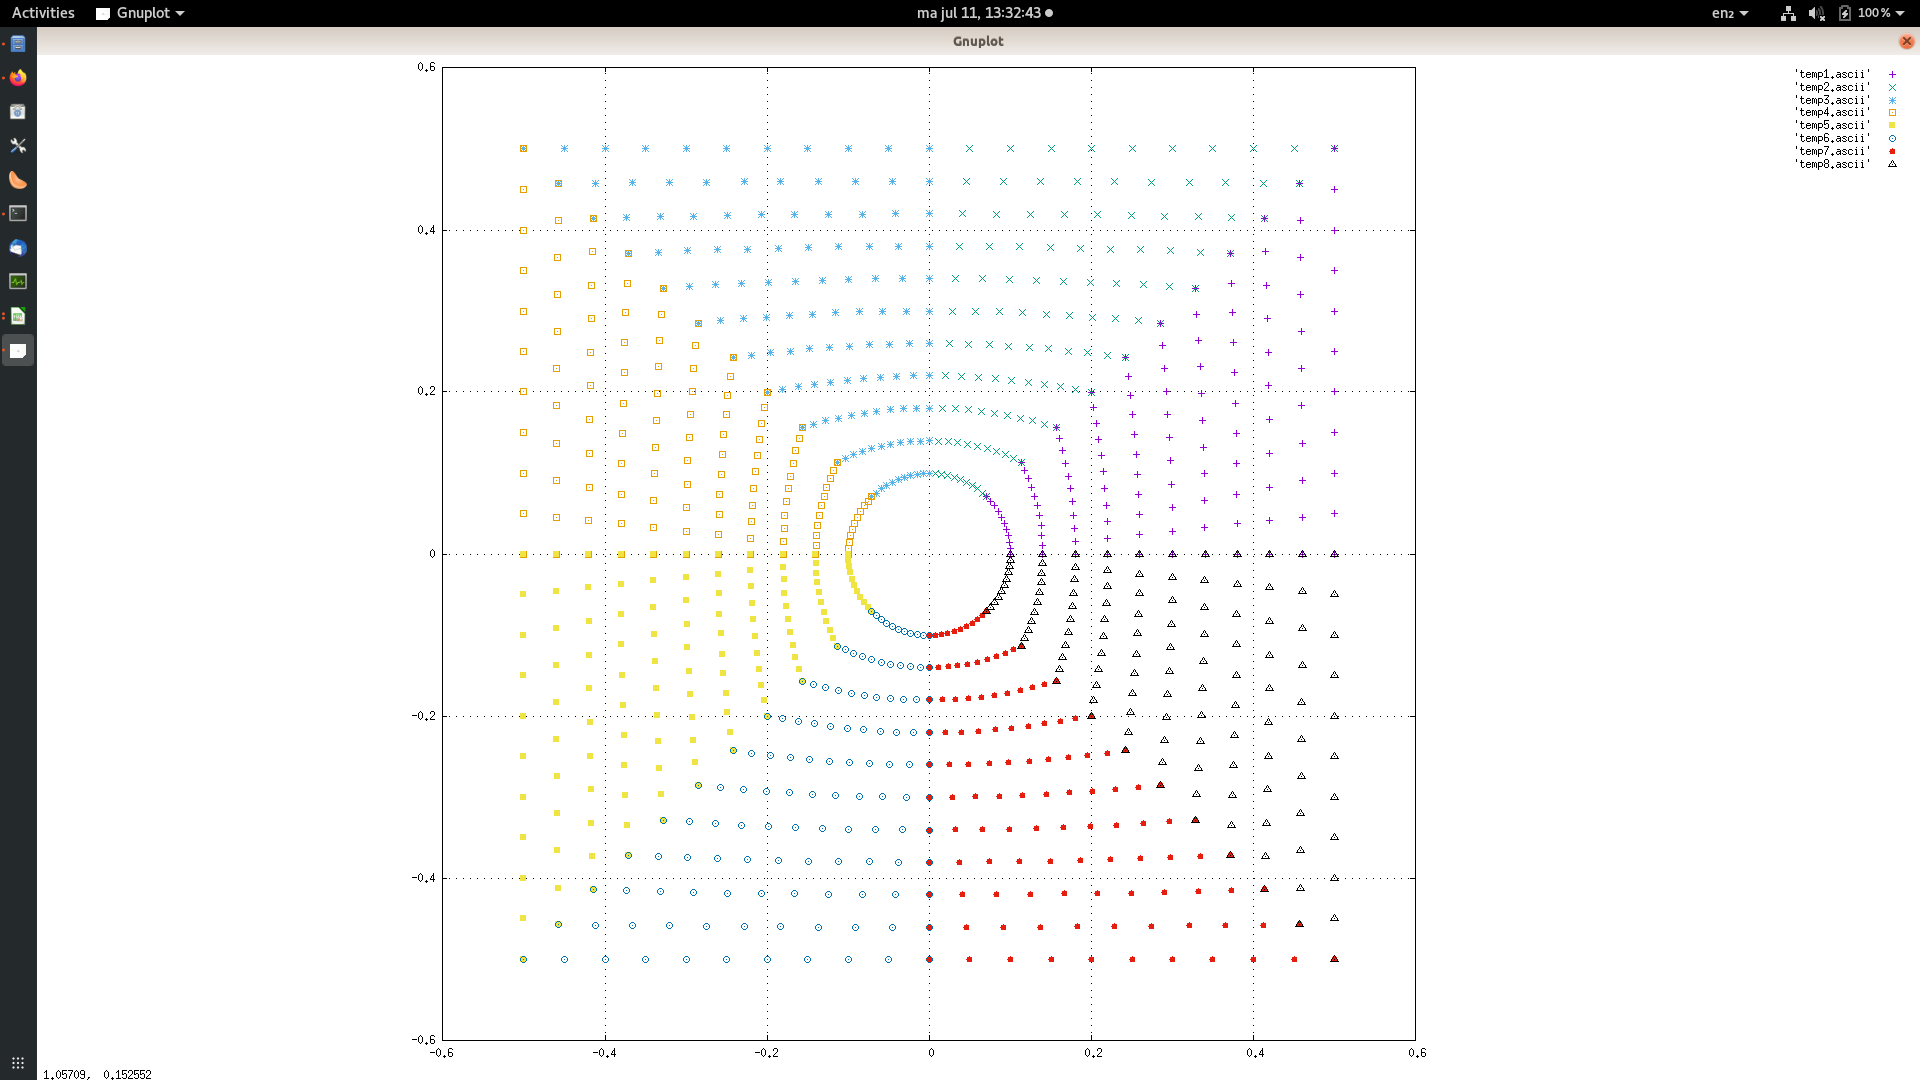
\includegraphics[width=12cm]{python_codes/fieldstone_124/results/mesh1}
\end{center}

Blocks 1 and 2 (purple and green respectively) are made from a regular $nelx\times nely$ mesh that is 
mapped to conform to the desired shape. Blocks 3 to 8 are rotations 
of either block 1 or 2. Note that in the current version $nelx$ and
$nely$ should be equal.
When all 8 blocks are obtained nodes which appear twice are removed
and a global connectivity array is made: 

\begin{center}
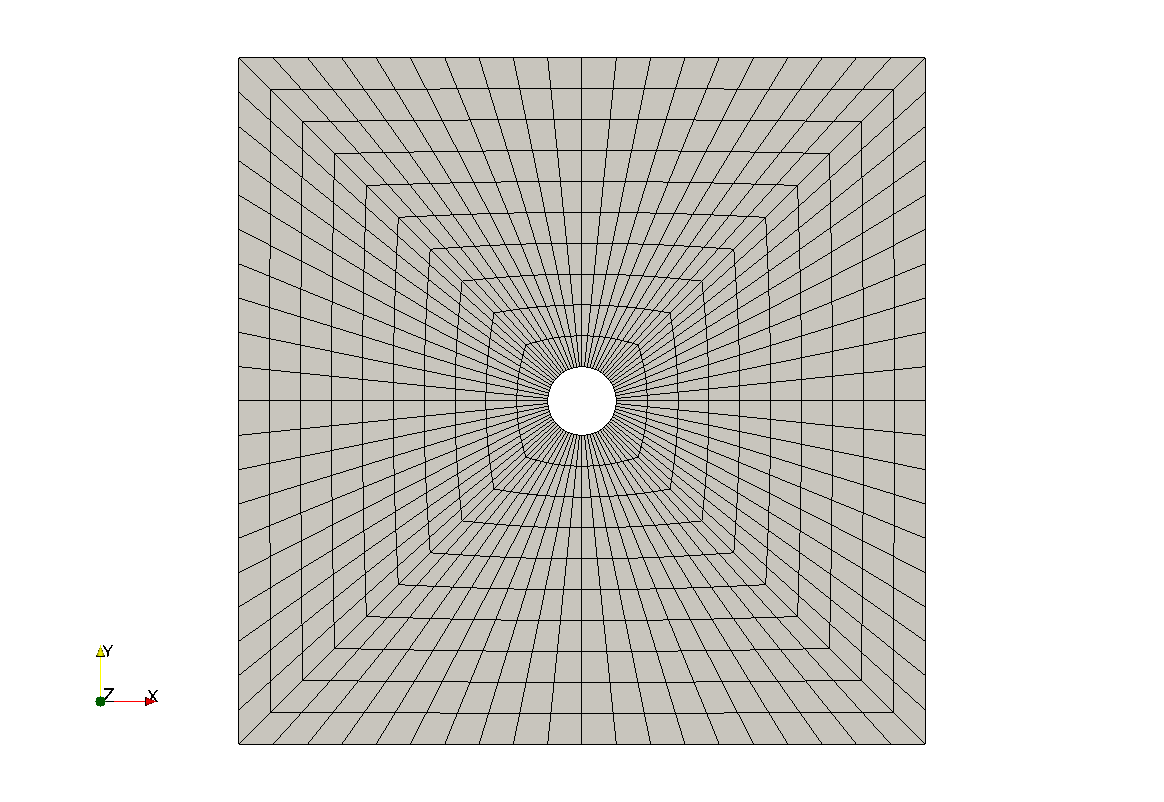
\includegraphics[width=8cm]{python_codes/fieldstone_124/results/mesh2}
\end{center}

This is unfortunately a rather slow algorithm and it will take 
several minutes to generate a mesh for $nelx$ values above 60.

\newpage
%--------------------------------------------------------------
\subsection*{Hassani experiment (experiment=1)}

This is taken from Prof. Hassani's syllabus 'Mise en oeuvre de la m\'ethode des \'el\'ements finis'.
The domain is a plate of $1\times 1~\si{\meter}$ with a $0.2~\si{\meter}$ diameter hole in its center.
Vertical displacements $\pm \upupsilon_0$ are prescribed on the top and bottom surface while 
the horizontal displacements are left free. No boundary condition is prescribed on the hole (i.e.
${\bm \sigma}\cdot \vec{n}=\vec{0}$).
In order to remove the translational nullspace, we impose $\upupsilon_x=0$
at $(x=0.5,y=0)$. Material properties are indicated on the following figure.

\begin{center}
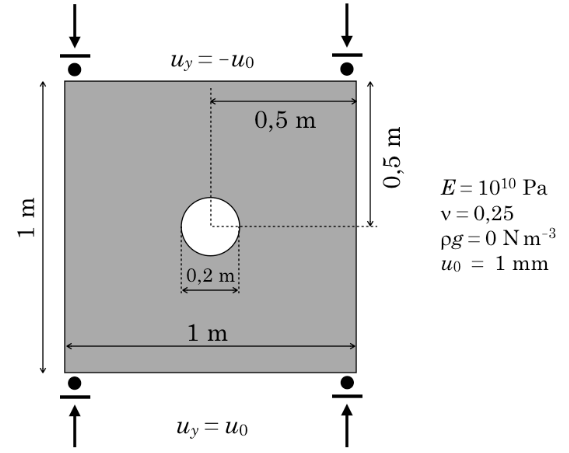
\includegraphics[width=5.8cm]{python_codes/fieldstone_124/images/hassani1}
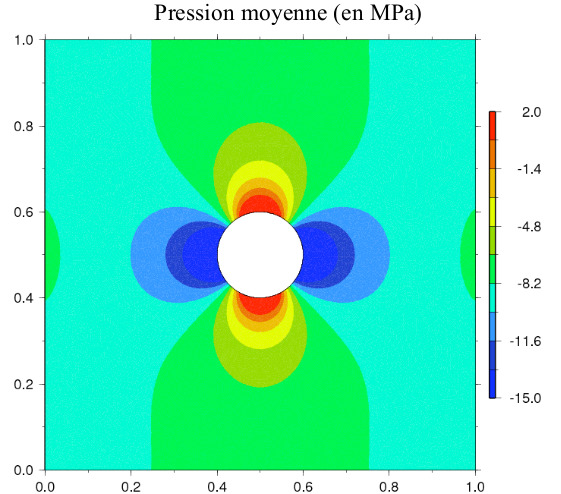
\includegraphics[width=5.2cm]{python_codes/fieldstone_124/images/hassani2}
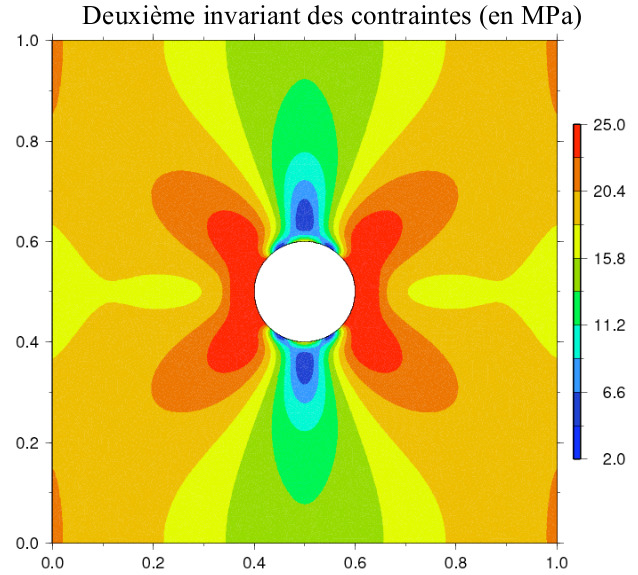
\includegraphics[width=5cm]{python_codes/fieldstone_124/images/hassani3}\\
{\captionfont Taken from Prof. Hassani's syllabus. Note that pressure in this plot is the opposite 
of our pressure (different convention). Also, it is not exactly clear 
which exact invariant was used in the right plot (private comm.).}
\end{center}

\begin{center}
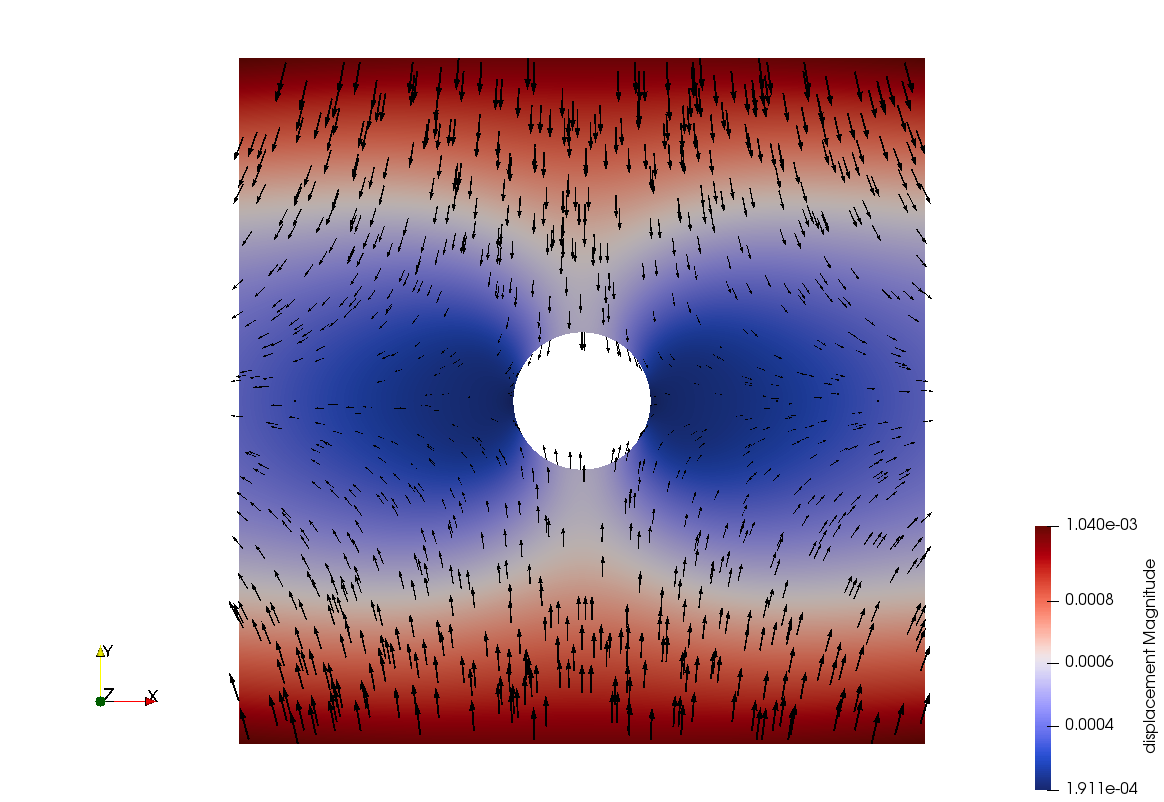
\includegraphics[width=5.6cm]{python_codes/fieldstone_124/results/exp1/disp}
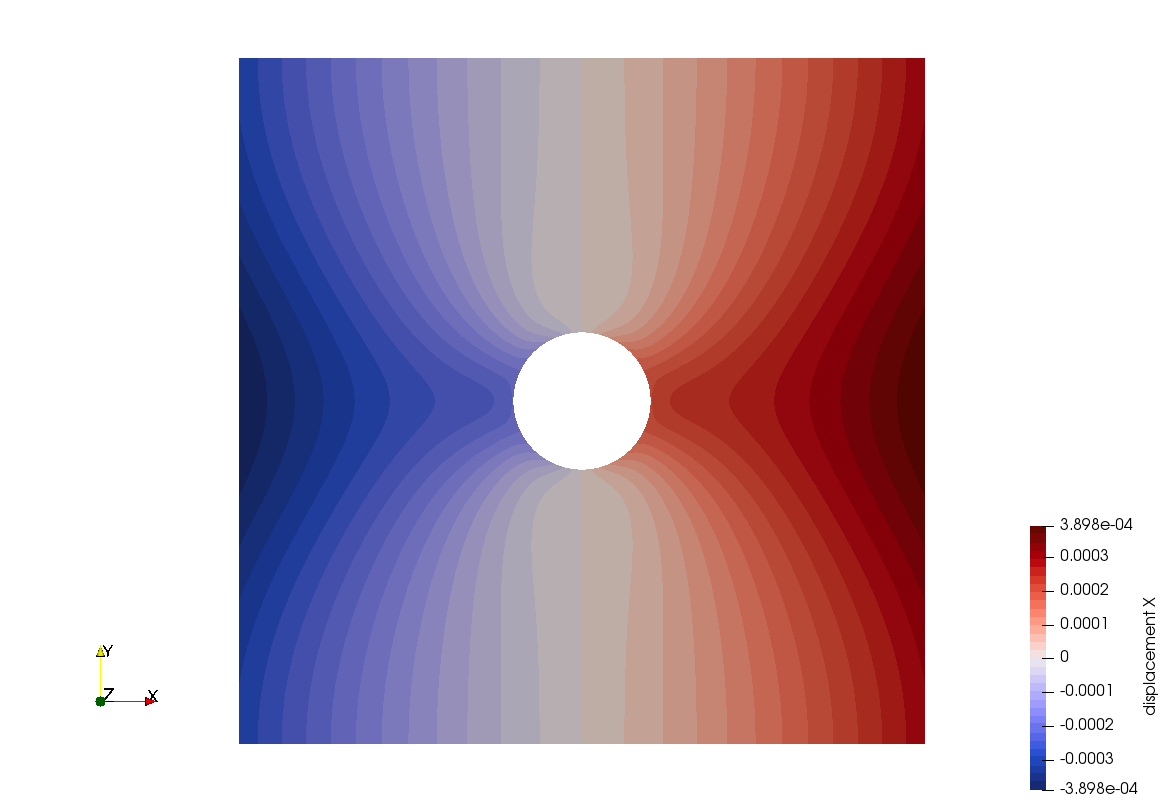
\includegraphics[width=5.6cm]{python_codes/fieldstone_124/results/exp1/disp_x}
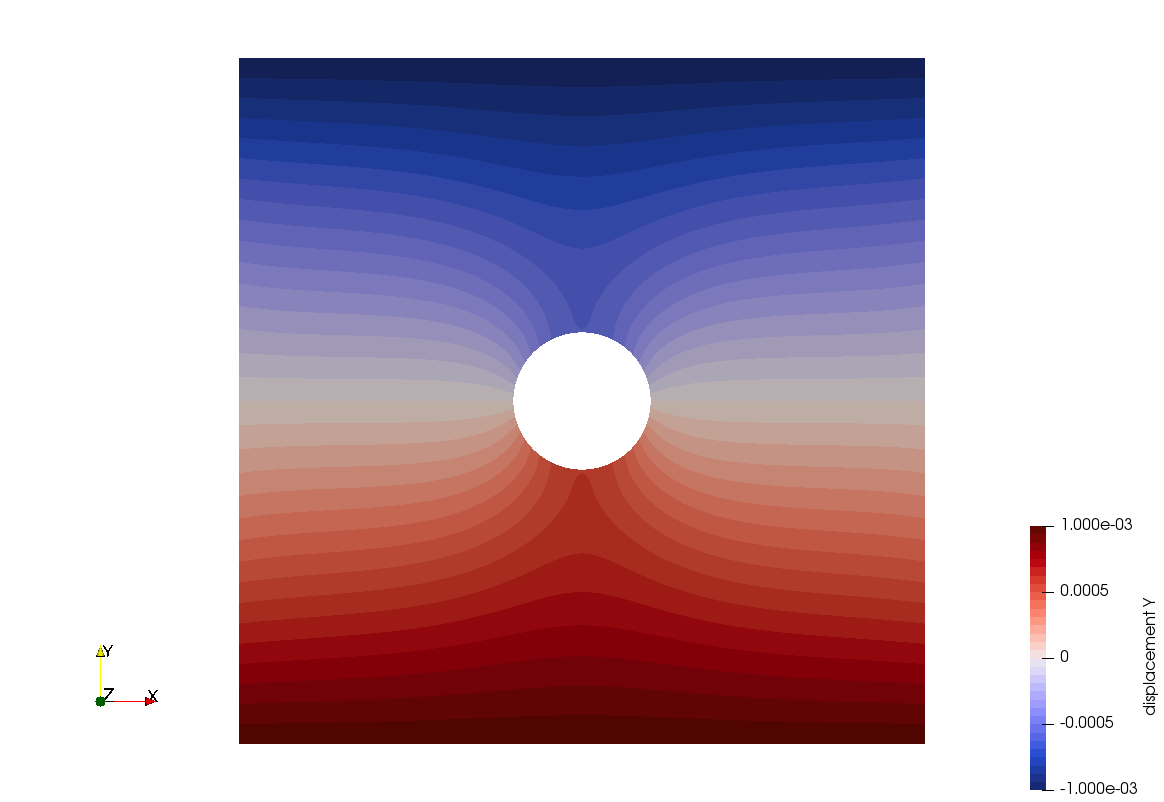
\includegraphics[width=5.6cm]{python_codes/fieldstone_124/results/exp1/disp_y}\\
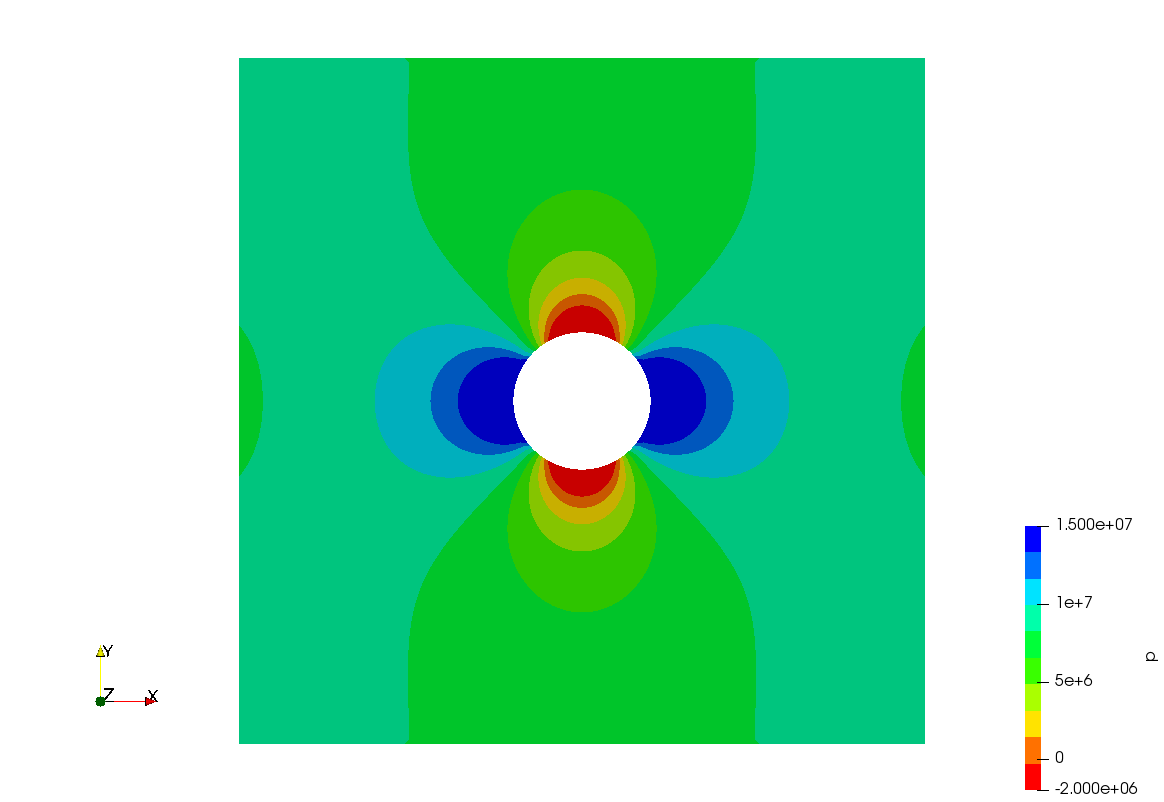
\includegraphics[width=5.6cm]{python_codes/fieldstone_124/results/exp1/press}
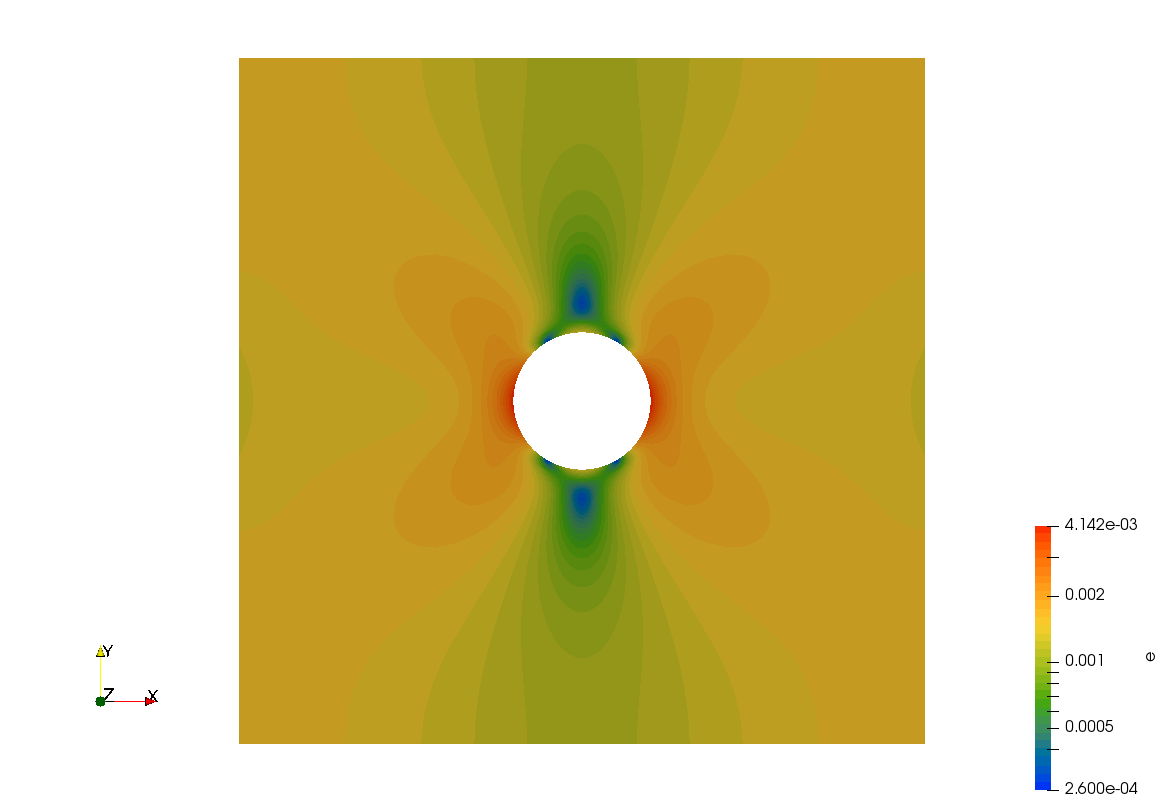
\includegraphics[width=5.6cm]{python_codes/fieldstone_124/results/exp1/e}
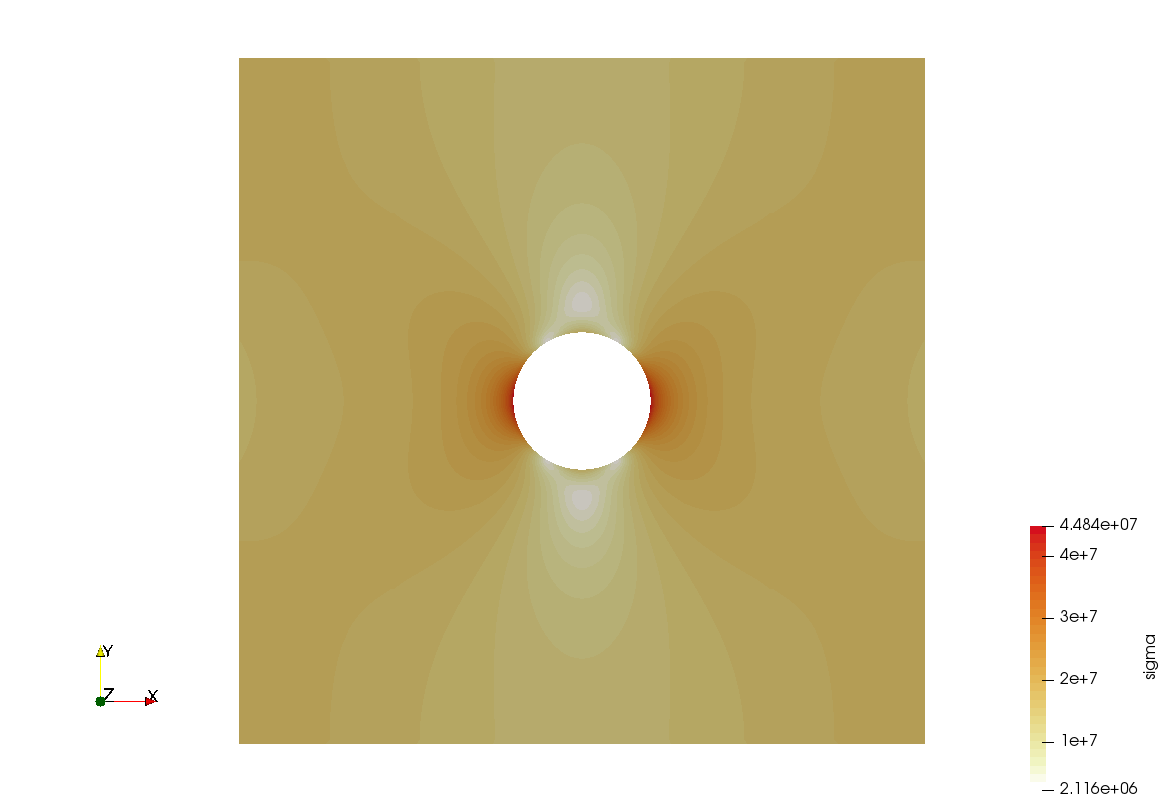
\includegraphics[width=5.6cm]{python_codes/fieldstone_124/results/exp1/sigma}\\
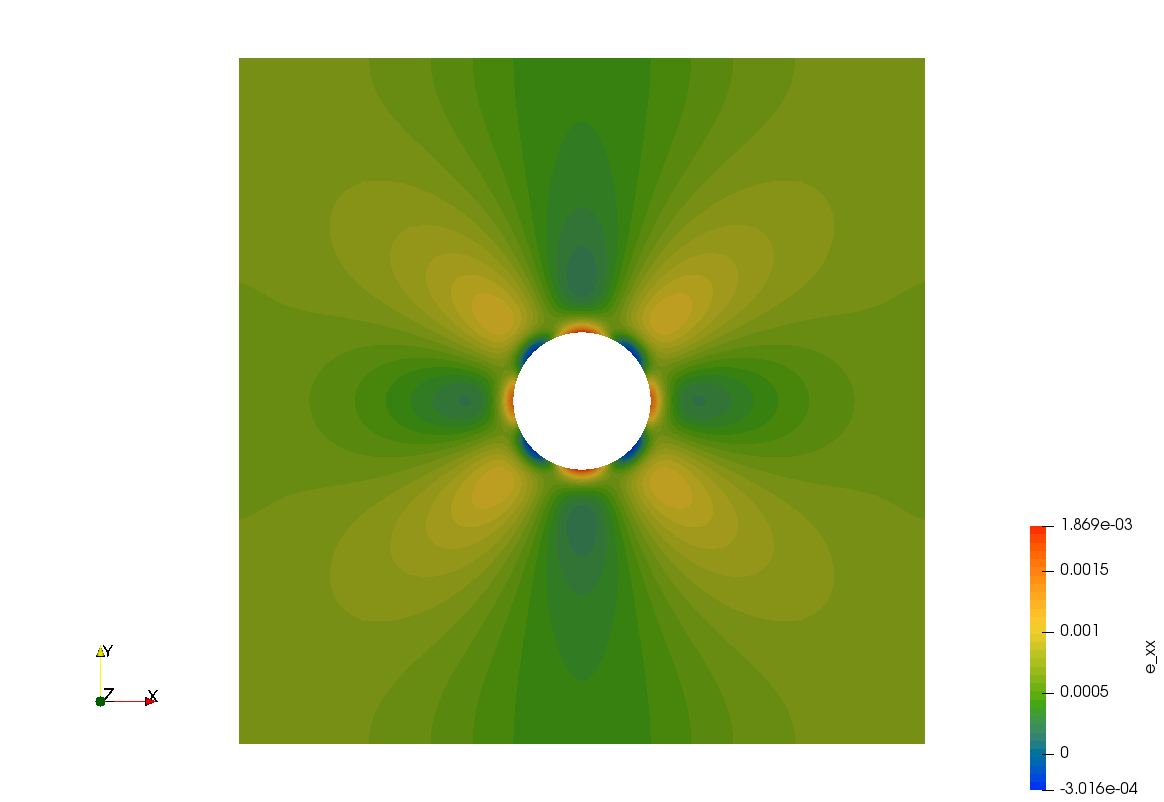
\includegraphics[width=5.6cm]{python_codes/fieldstone_124/results/exp1/exx}
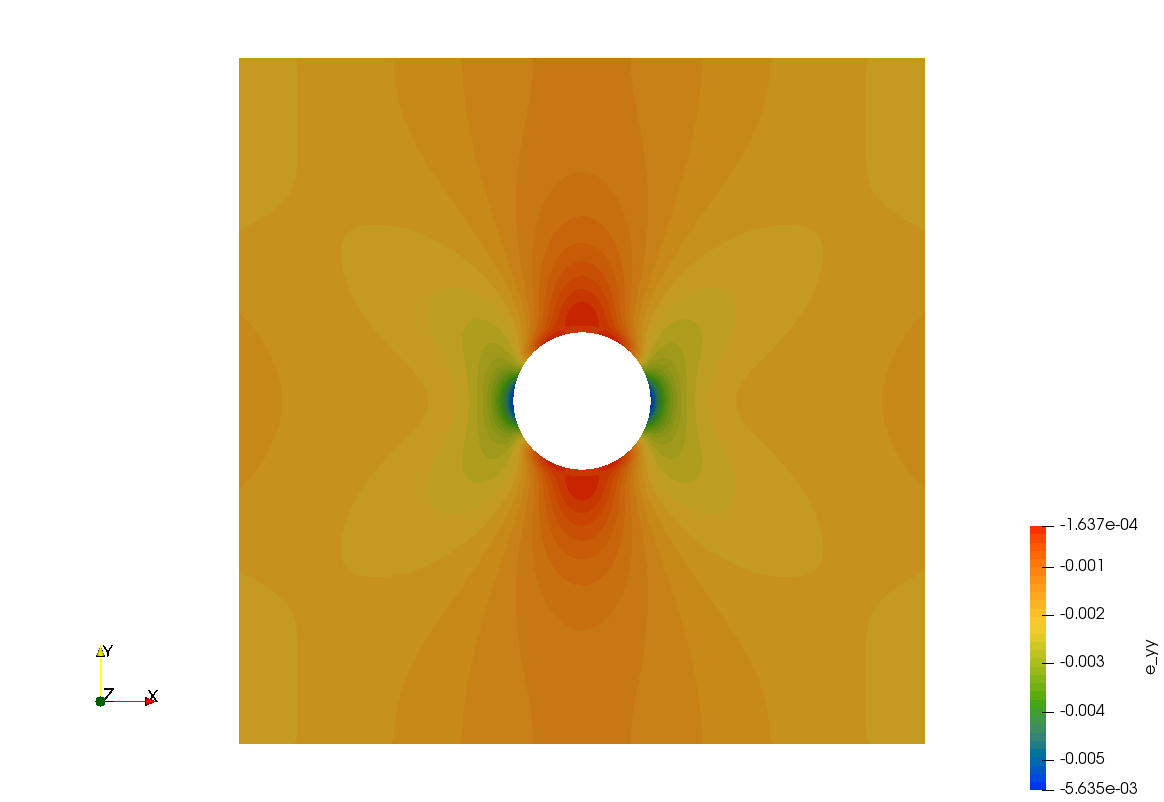
\includegraphics[width=5.6cm]{python_codes/fieldstone_124/results/exp1/eyy}
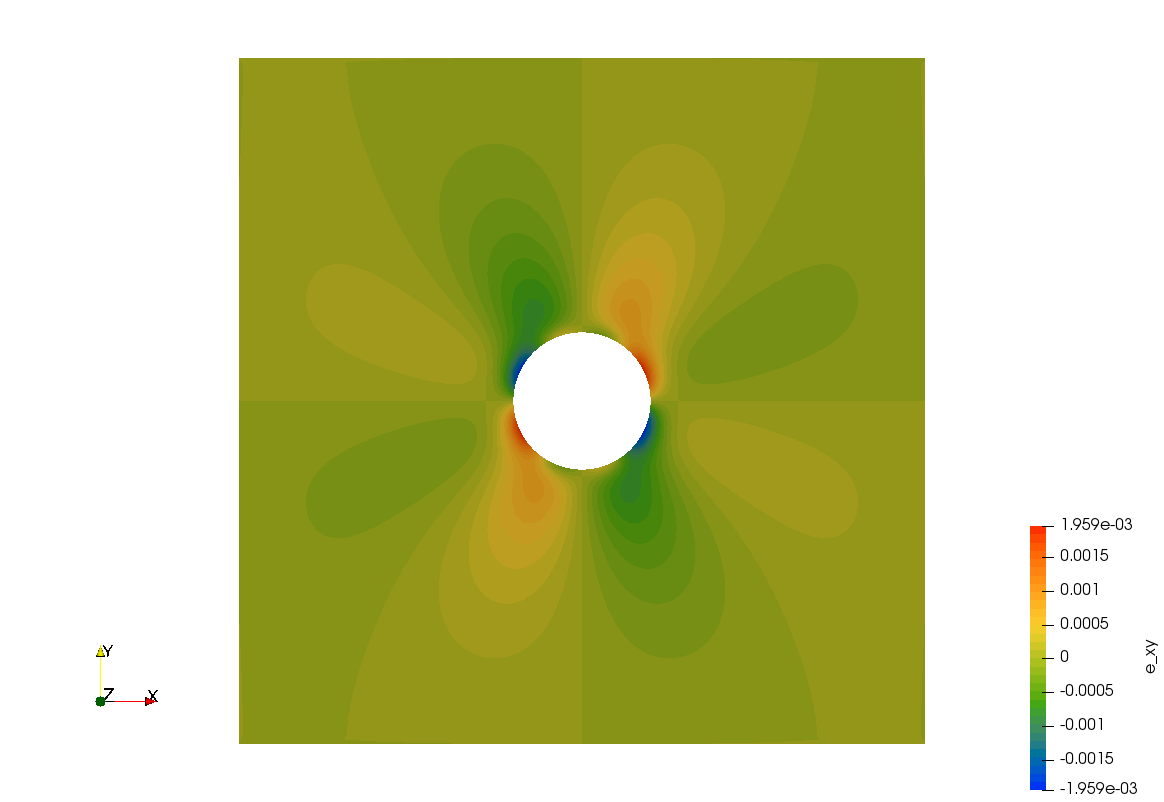
\includegraphics[width=5.6cm]{python_codes/fieldstone_124/results/exp1/exy}\\
{\captionfont Each block counts $64\times 64$ elements. Exceptionally a rainbow
color scale is used for the pressure so as to allow for a comparison with 
the figure from Hassani.}
\end{center}


\begin{center}
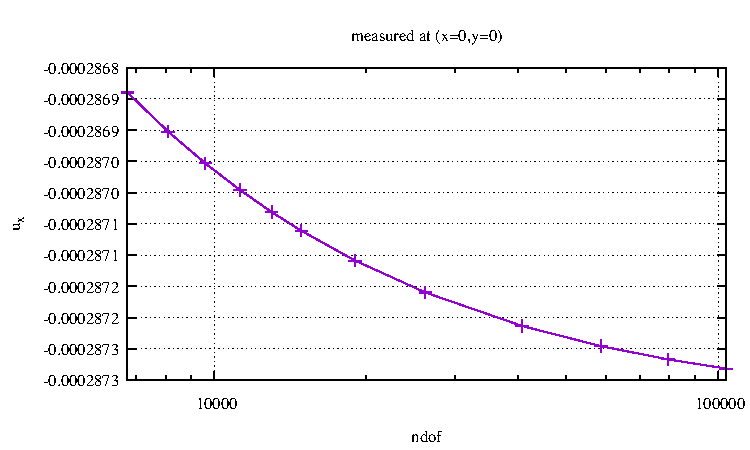
\includegraphics[width=5.6cm]{python_codes/fieldstone_124/results/exp1/corner_ux}
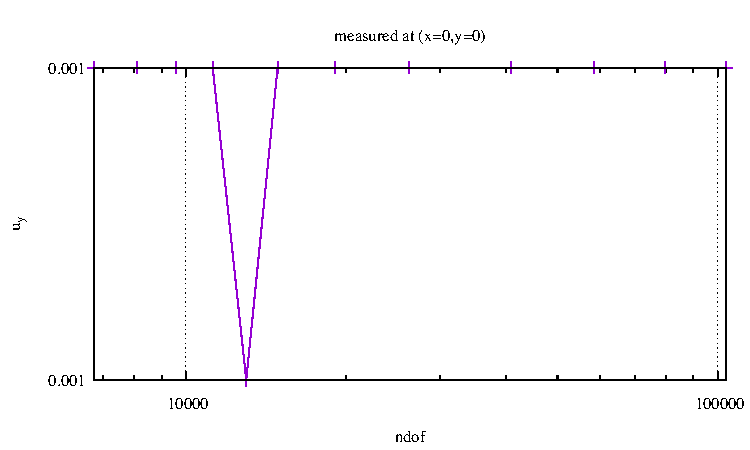
\includegraphics[width=5.6cm]{python_codes/fieldstone_124/results/exp1/corner_uy}
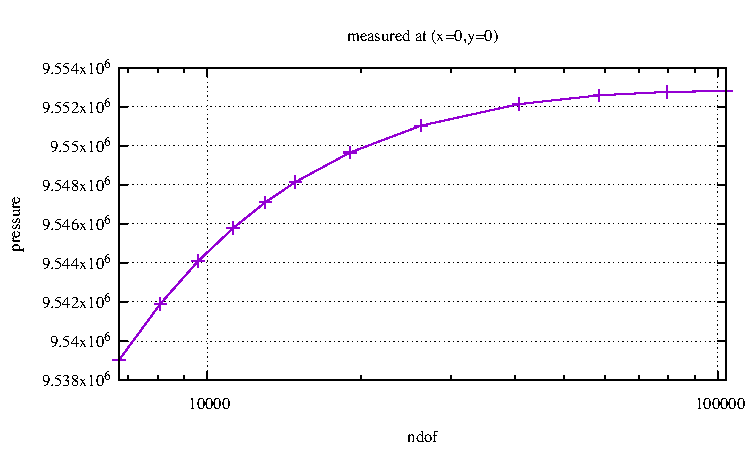
\includegraphics[width=5.6cm]{python_codes/fieldstone_124/results/exp1/corner_p}\\
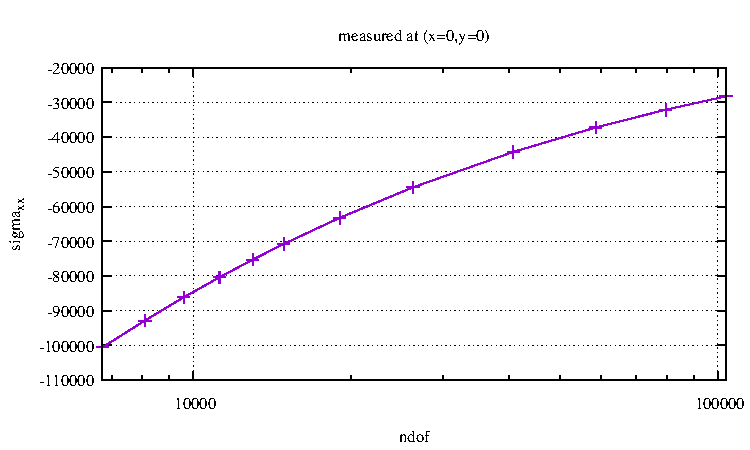
\includegraphics[width=5.6cm]{python_codes/fieldstone_124/results/exp1/corner_sigmaxx}
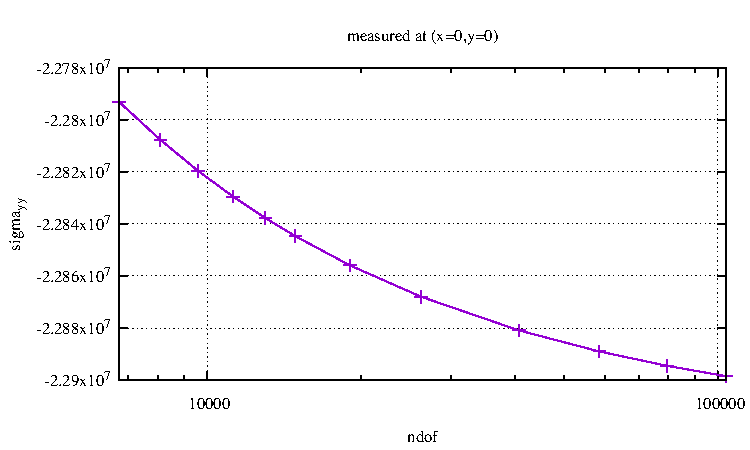
\includegraphics[width=5.6cm]{python_codes/fieldstone_124/results/exp1/corner_sigmayy}
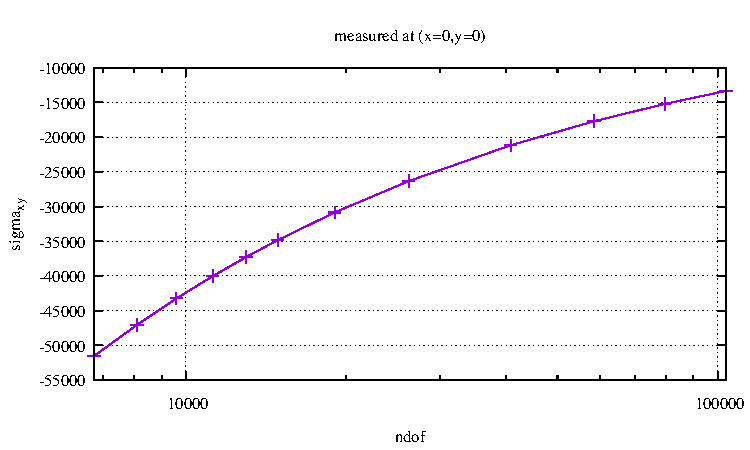
\includegraphics[width=5.6cm]{python_codes/fieldstone_124/results/exp1/corner_sigmaxy}\\
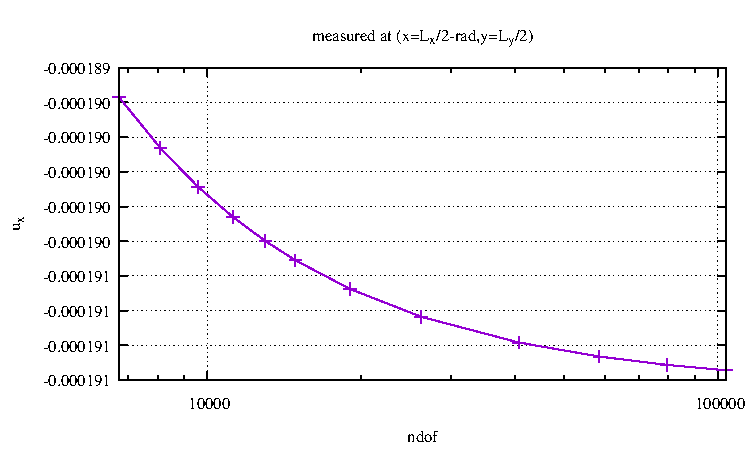
\includegraphics[width=5.6cm]{python_codes/fieldstone_124/results/exp1/west_ux}
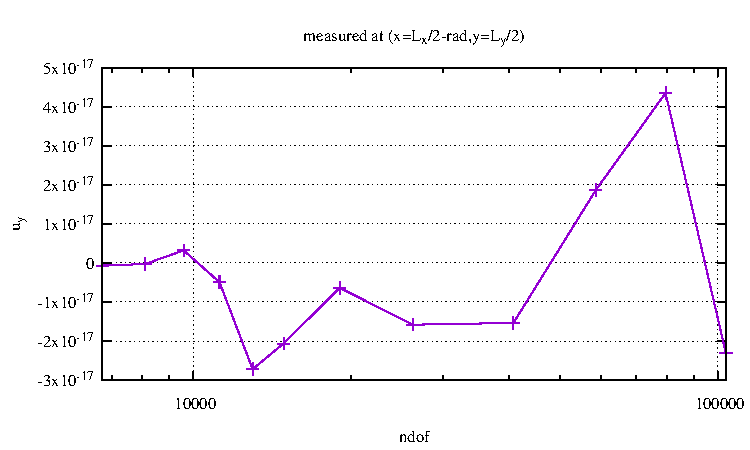
\includegraphics[width=5.6cm]{python_codes/fieldstone_124/results/exp1/west_uy}
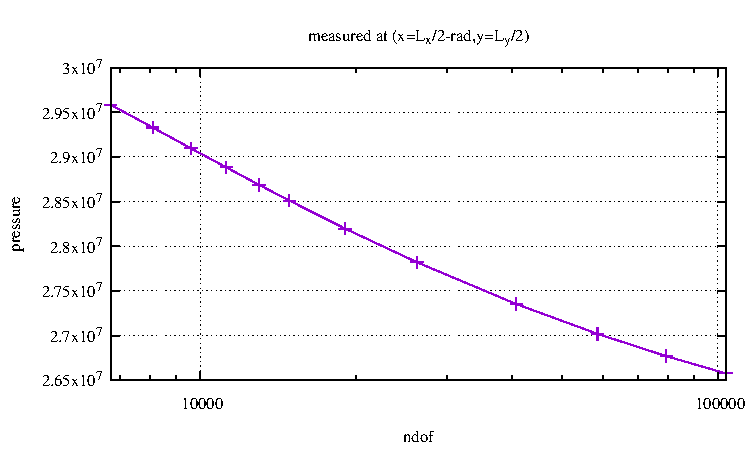
\includegraphics[width=5.6cm]{python_codes/fieldstone_124/results/exp1/west_p}\\
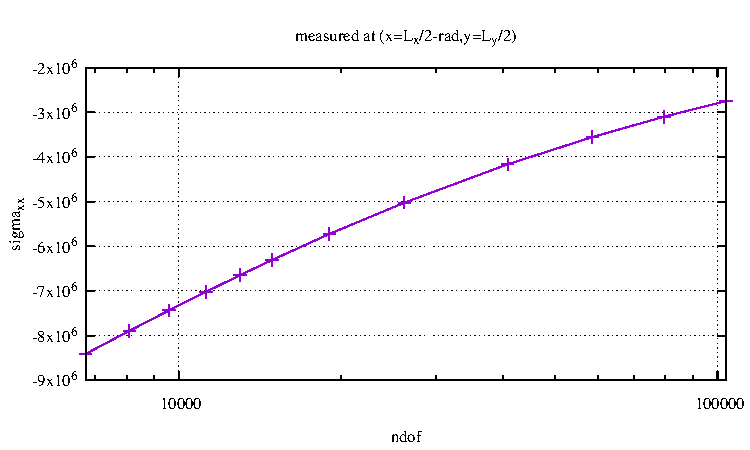
\includegraphics[width=5.6cm]{python_codes/fieldstone_124/results/exp1/west_sigmaxx}
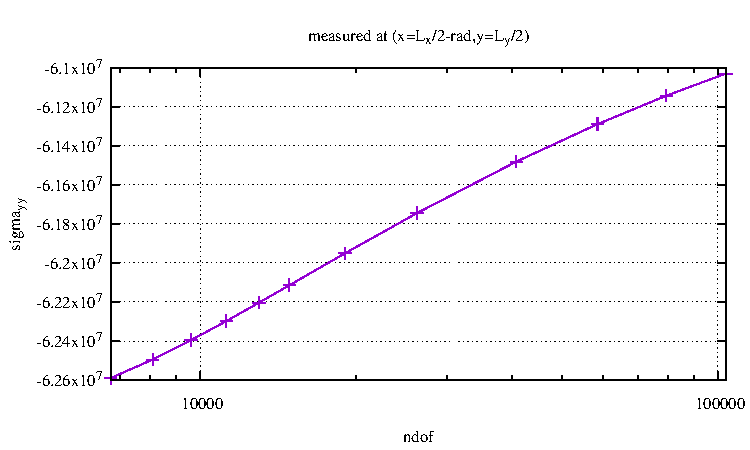
\includegraphics[width=5.6cm]{python_codes/fieldstone_124/results/exp1/west_sigmayy}
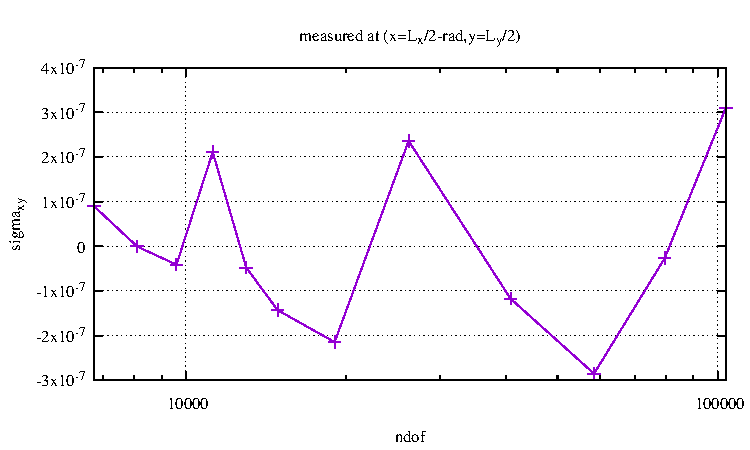
\includegraphics[width=5.6cm]{python_codes/fieldstone_124/results/exp1/west_sigmaxy}\\
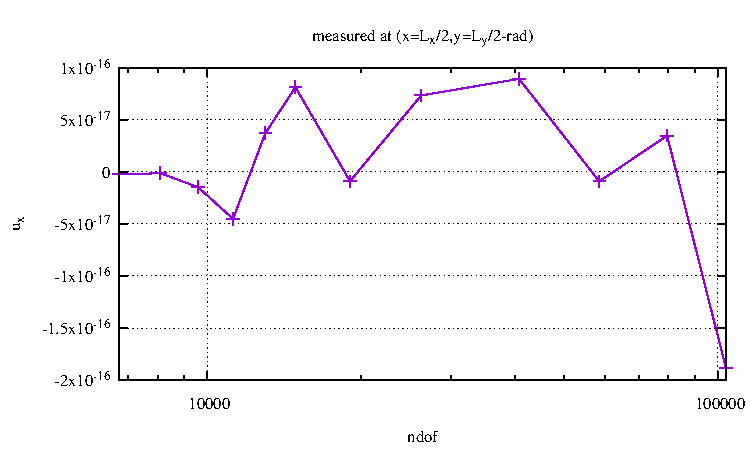
\includegraphics[width=5.6cm]{python_codes/fieldstone_124/results/exp1/south_ux}
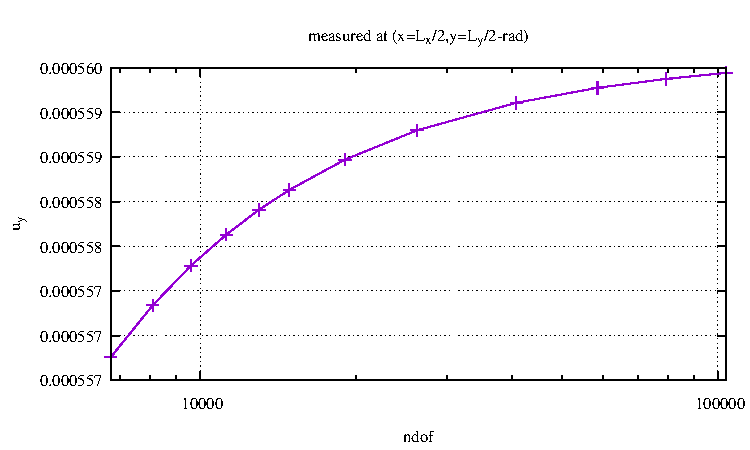
\includegraphics[width=5.6cm]{python_codes/fieldstone_124/results/exp1/south_uy}
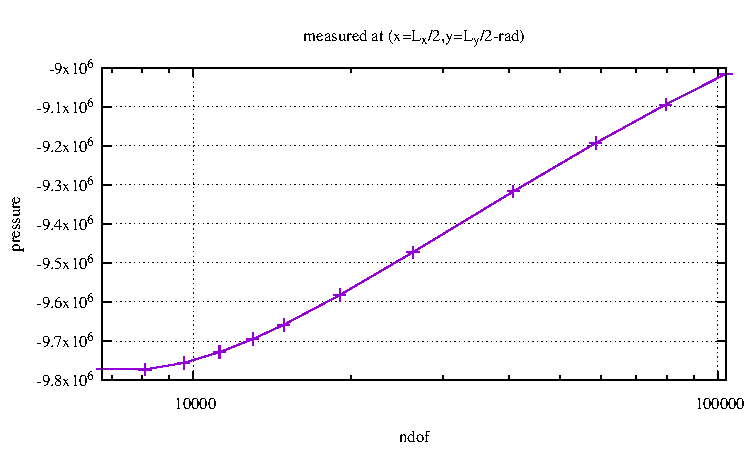
\includegraphics[width=5.6cm]{python_codes/fieldstone_124/results/exp1/south_p}\\
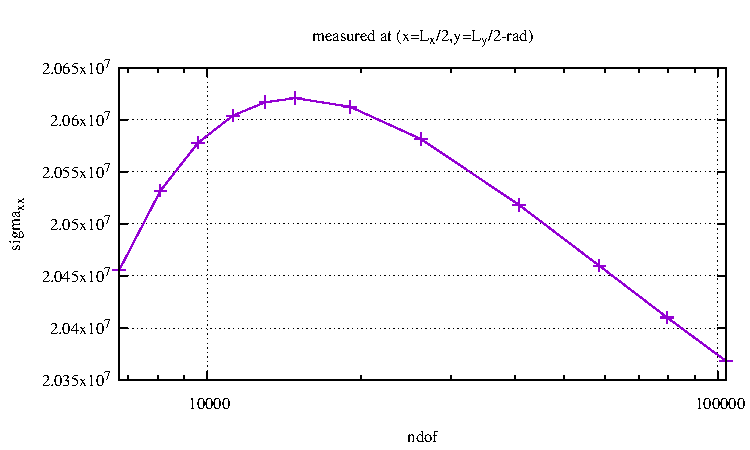
\includegraphics[width=5.6cm]{python_codes/fieldstone_124/results/exp1/south_sigmaxx}
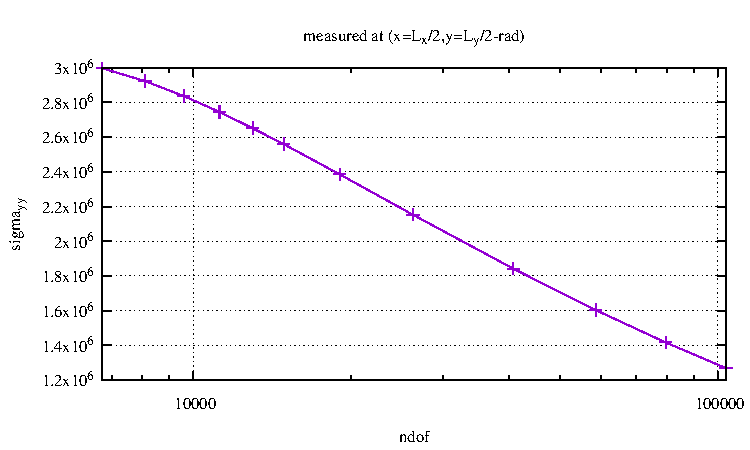
\includegraphics[width=5.6cm]{python_codes/fieldstone_124/results/exp1/south_sigmayy}
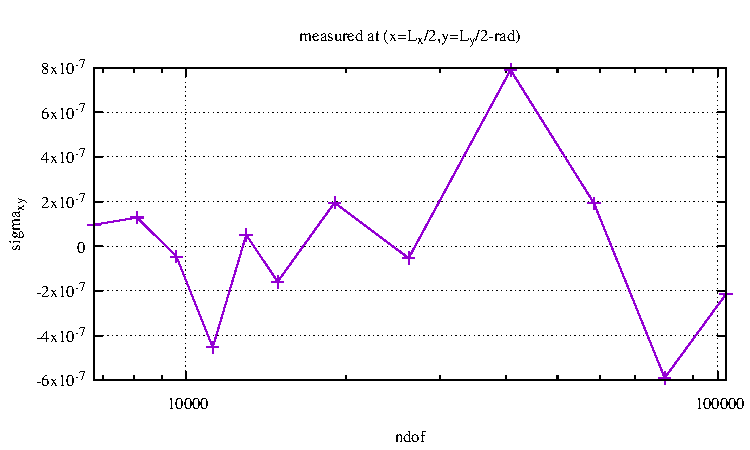
\includegraphics[width=5.6cm]{python_codes/fieldstone_124/results/exp1/south_sigmaxy}
\end{center}






\newpage
%--------------------------------------------------------------
\subsection*{\textcite{rama16} (experiment=2)}

An infinite plate with a circular hole of radius $a$  
is subjected to a unidirectional tensile load of $\sigma$ in the $x$ direction as shown
in the figure. In this case, only one quarter of the domain could be analysed due
to symmetry along $x$ and $y$ axis but we nevertheless model the full plate.

\begin{center}
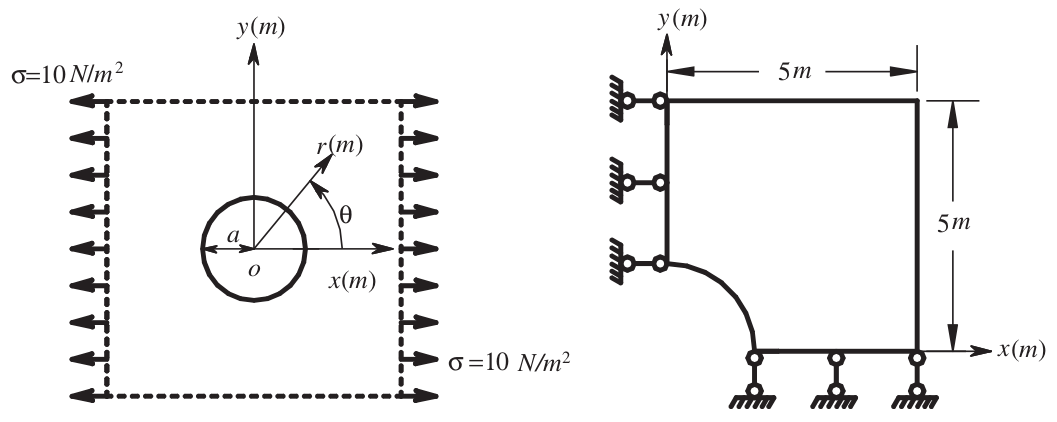
\includegraphics[width=0.65\textwidth]{python_codes/fieldstone_124/images/yobu02}
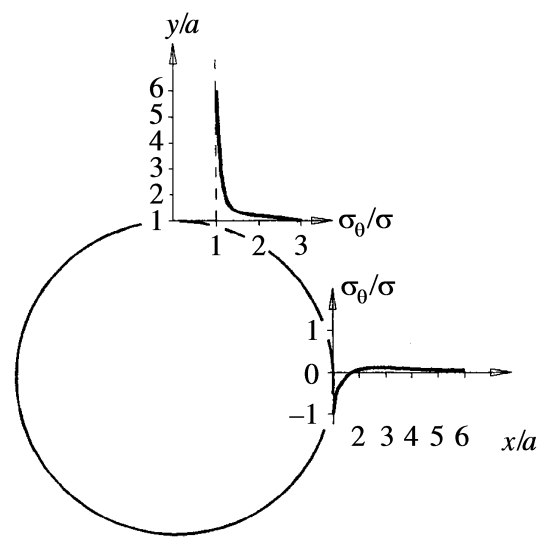
\includegraphics[width=0.25\textwidth]{python_codes/fieldstone_124/images/yobu02b}
{\captionfont Left: An infinite plate with a circular hole subjected to unidirectional tension 
and its quarter model with symmetric conditions imposed on the left and bottom edges.
Right: Tangential stress distribution for $\theta=0$  and $\theta=\pi/2$. \cite{yobu02}}
\end{center}


The inner boundary of the hole is traction free. 
On the left and right edges tractions based on the analytical solutions are prescribed.
The {\color{red}plane stress} condition is considered and the parameters are: 
Young modulus $E=\SI{3e7}{\mega\pascal}$, Poisson Ratio $\nu=0.3$, 
Load $\sigma=10~\si{\newton\per\square\meter}$, $a=1~\si{\meter}$.

The analytical stress components for this problem are  

\begin{eqnarray}
\sigma_{xx}(x,y) &=& \sigma \left(  1-\frac{a^2}{r^2}\left(\frac{3}{2}\cos 2\theta + \cos 4\theta \right) 
+ \frac{3a^4}{2r^4} \cos 4\theta \right) \\
\sigma_{yy}(x,y) &=& -\sigma \left( \frac{a^2}{r^2} \left(\frac{1}{2}\cos 2\theta - \cos 4\theta \right) 
- \frac{3a^4}{2r^4} \cos 4\theta \right) \\
\sigma_{xy}(x,y) &=& -\sigma \left( \frac{a^2}{r^2} \left(\frac{1}{2}\sin 2\theta + \sin 4\theta\right) 
+ \frac{3a^4}{2r^4} \sin 4\theta \right) 
\end{eqnarray}

Note that on page 31 of \textcite{rama16} (2016) cites \textcite{chnn10} (2010)
which cites the book \cite[p772]{yobu02} which cites \textcite{budynas} for the solution!
\todo[inline]{there are discrepancies between \cite{rama16} and \cite{chnn10}. because of course.}

Following \cite{yobu02}, it can be shown, from linear elasticity, that the tangential
stress throughout the plate is given by
\[
\sigma_\theta = \frac{\sigma}{2} \left[ 1+\frac{a^2}{r^2} - 
\left( 1+3\frac{a^4}{r^4}  \right) \cos 2\theta   \right]
\]
The maximum stress is $\sigma_\theta=3\sigma$ at $r=a$ and $\theta=\pm \pi/2$. Along the surface of the hole, 
the tangential stress is $-\sigma$ at y $\theta=0$  and $\theta=\pi$, 
and increases, as $\theta$ increases, to $3\sigma$ at $\theta=\pi/2$ and $\theta=3\pi/2$.



























\newpage
%--------------------------------------------------------------
\subsection*{\textcite{rarr03} (experiment=3)}

This is section~11.2.2 of the book.
The benchmark consists of a stretched plate with a circular central hole under plane strain condition. 
The width $b$ of the plate is 
equal to its height $h = \SI{100}{\mm}$; the radius $r$ of the hole is \SI{10}{\mm}. 
The following figure shows the system with its boundary conditions. The applied tractions 
$\bar{p} = \SI{100}{\newton\per\square\mm}$ are scaled with the load factor\footnote{This has 
nothing to do with the real elastic parameter $\lambda$!} $\lambda=4.5$.
We use Young's modulus $E = \SI{206 900}{\kilo\newton\per\square\mm}$, and Poisson's ratio $\nu = 0.29$.

It is not clear what the boundary conditions are at the hole but we assume that no boundary
condition is prescribed, which is confirmed by the results that follow.
Because we model the whole plate we have $L_x=L_y=2h$.

There are two translational nullspaces and these are removed by 
prescribing horizontal or vertical displacements at key locations
where they have to be zero because of the symmetry of the problem.

\begin{center}
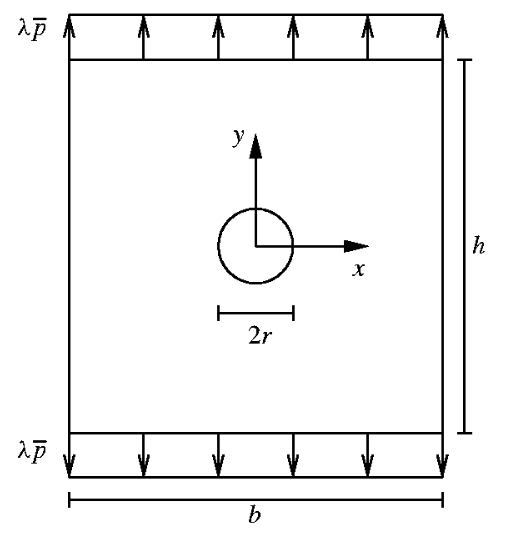
\includegraphics[width=5cm]{python_codes/fieldstone_124/images/rarr03a}
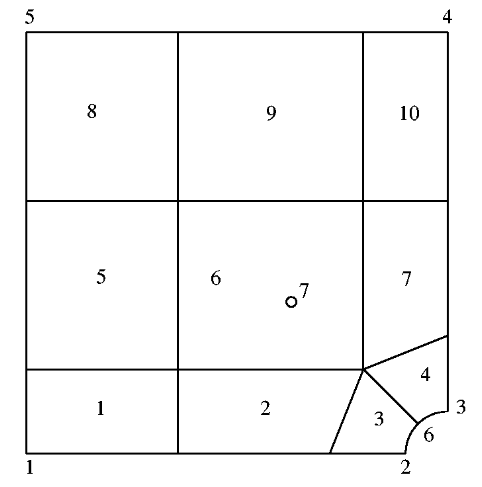
\includegraphics[width=5cm]{python_codes/fieldstone_124/images/rarr03c}
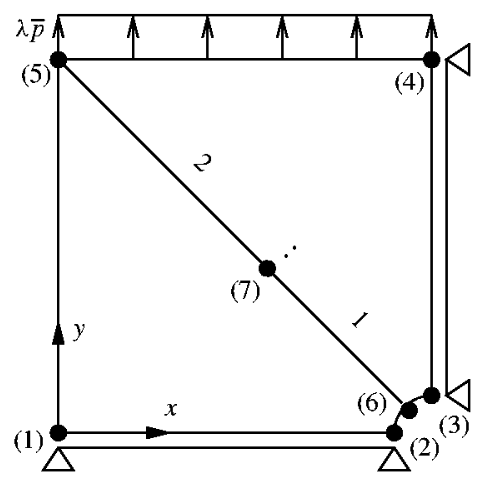
\includegraphics[width=5cm]{python_codes/fieldstone_124/images/rarr03f}\\
{\captionfont Taken from \textcite{rarr03}. In our domain 
Point (2) has coordinates $(L_x/2-rad,Ly/2)$,
Point (4) has coordinates $(L_x/2,Ly)$,
Point (5) has coordinates $(0,Ly)$.}
\end{center}

The following measurements are carried out:
\begin{itemize}
\item displacement $\upupsilon_x$ at point (2).
\item stress $\sigma_{yy}$  at point (2);
\item displacement $\upupsilon_y$ at point (4);
\item $\int_{(4)}^{(5)} \upupsilon_y$ (currently not implemented) 
\item displacement $\upupsilon_x$ at point (5);
\end{itemize}

Note that there seems to be a problem with the scaling of the results when the above 
parameters are used. Using instead $E=\SI{206 900}{\kilo\newton\per\square\meter}=2.069e8$
we recover the values of the following table: 
\begin{center}
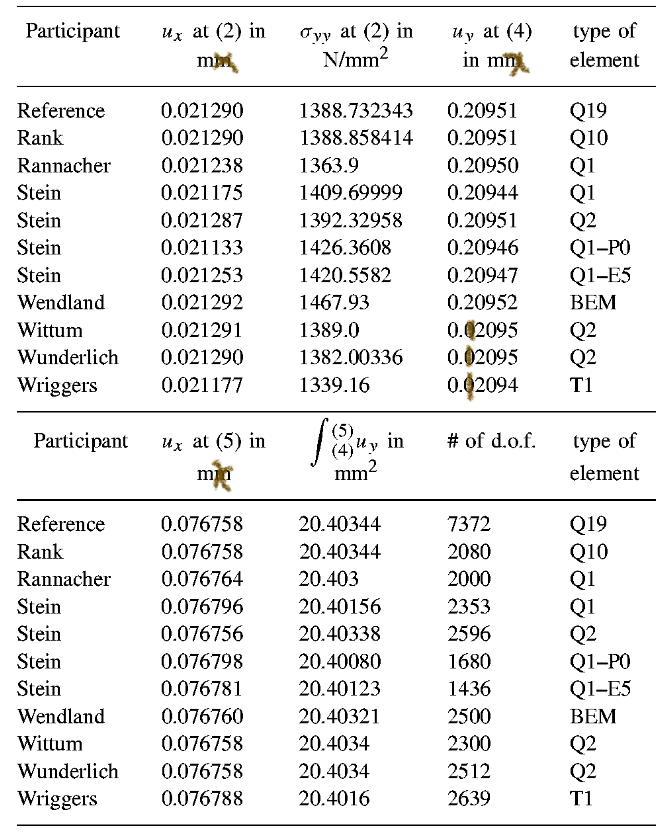
\includegraphics[width=8cm]{python_codes/fieldstone_124/images/rarr03b}\\
{\captionfont Taken from \textcite{rarr03}. Note that there probably is a 
problem with 3 values of the reported $\upupsilon_y$ for point (4).}
\end{center}


\begin{center}
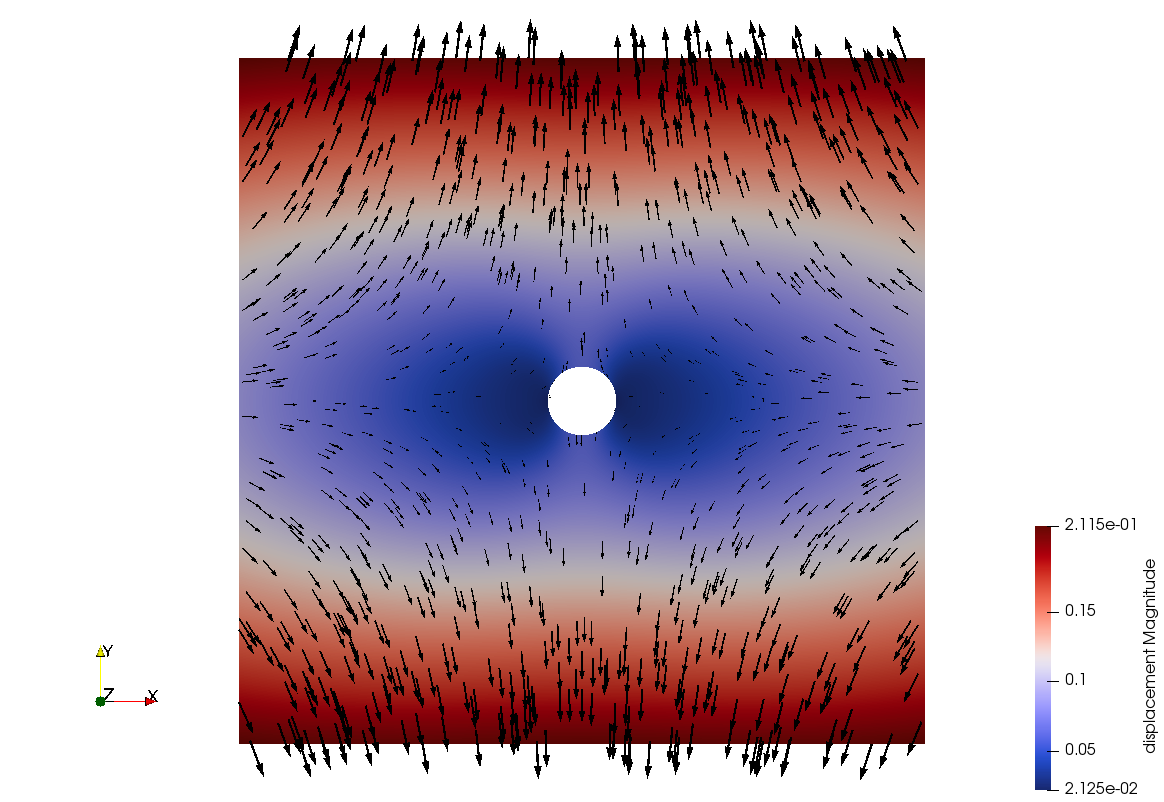
\includegraphics[width=5.6cm]{python_codes/fieldstone_124/results/exp3/disp}
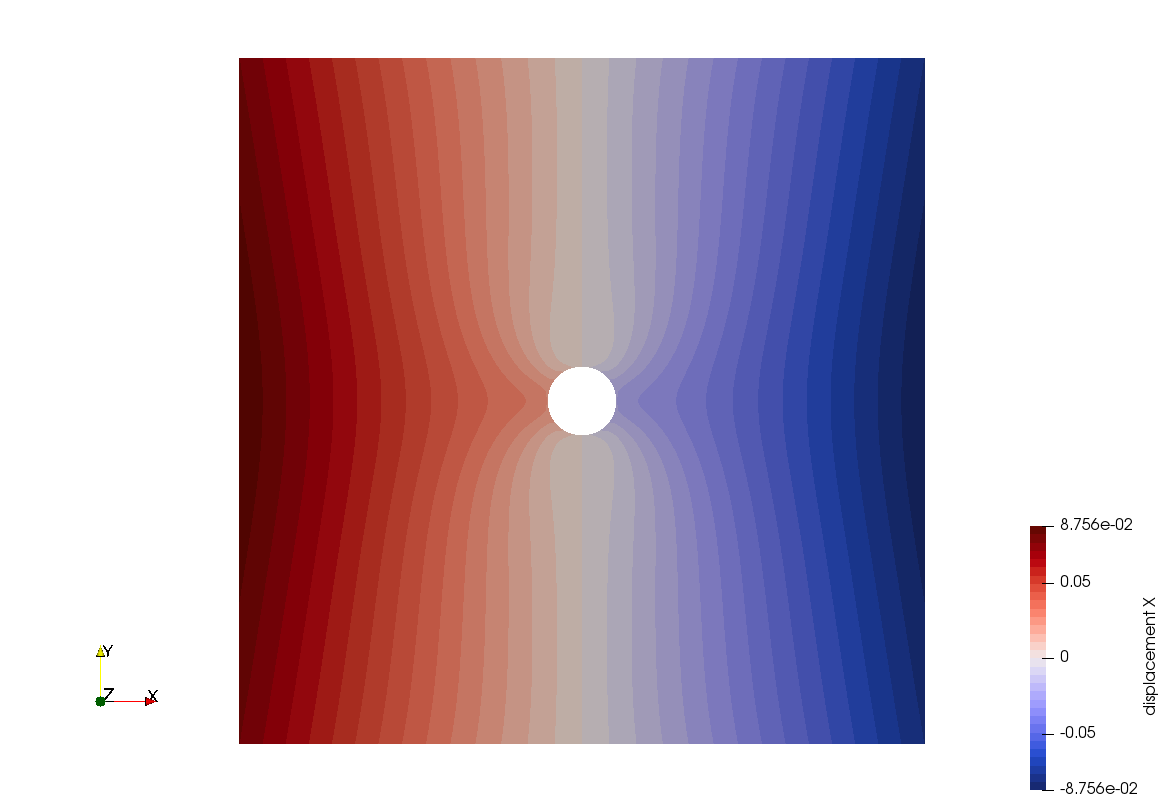
\includegraphics[width=5.6cm]{python_codes/fieldstone_124/results/exp3/disp_x}
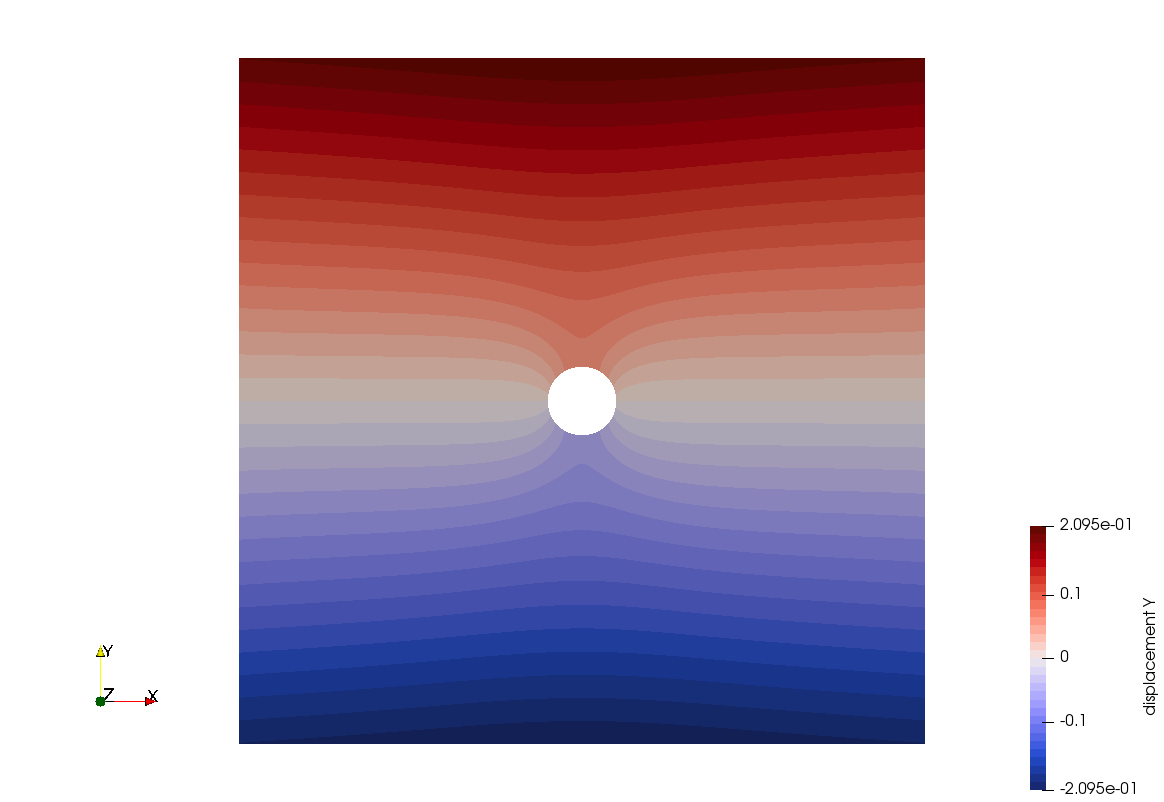
\includegraphics[width=5.6cm]{python_codes/fieldstone_124/results/exp3/disp_y}\\
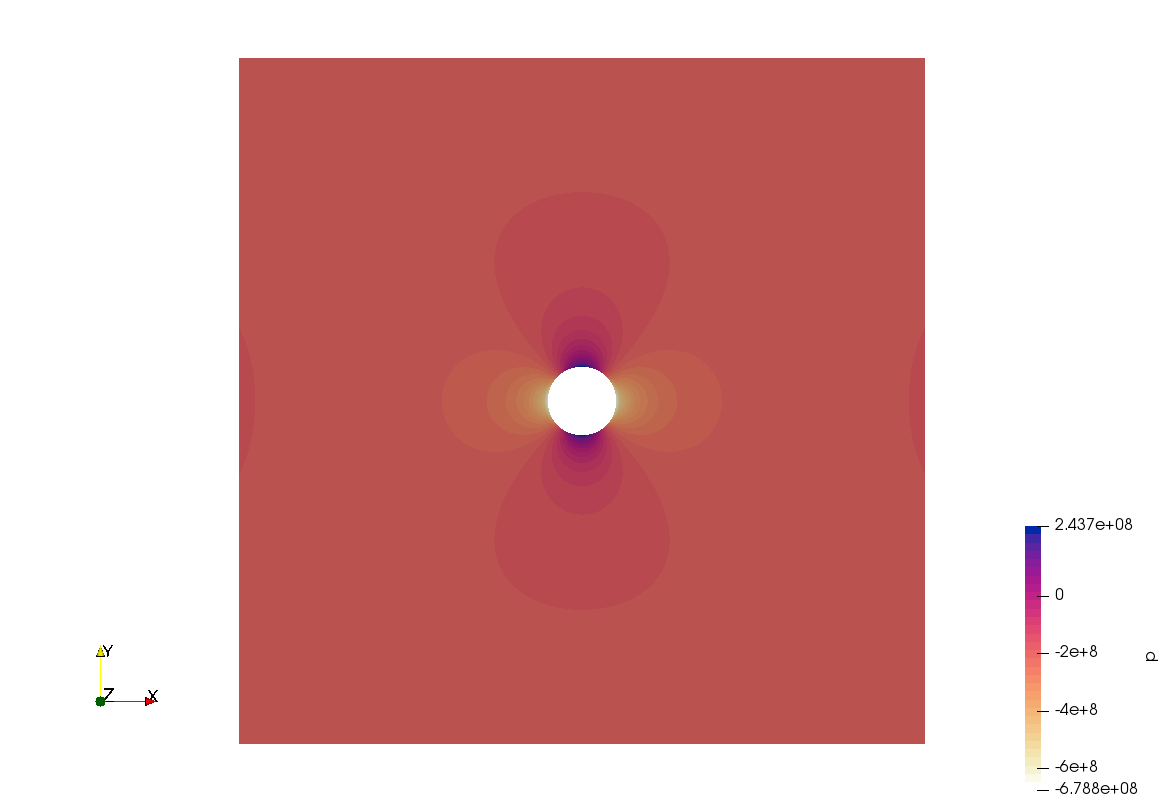
\includegraphics[width=5.6cm]{python_codes/fieldstone_124/results/exp3/press}
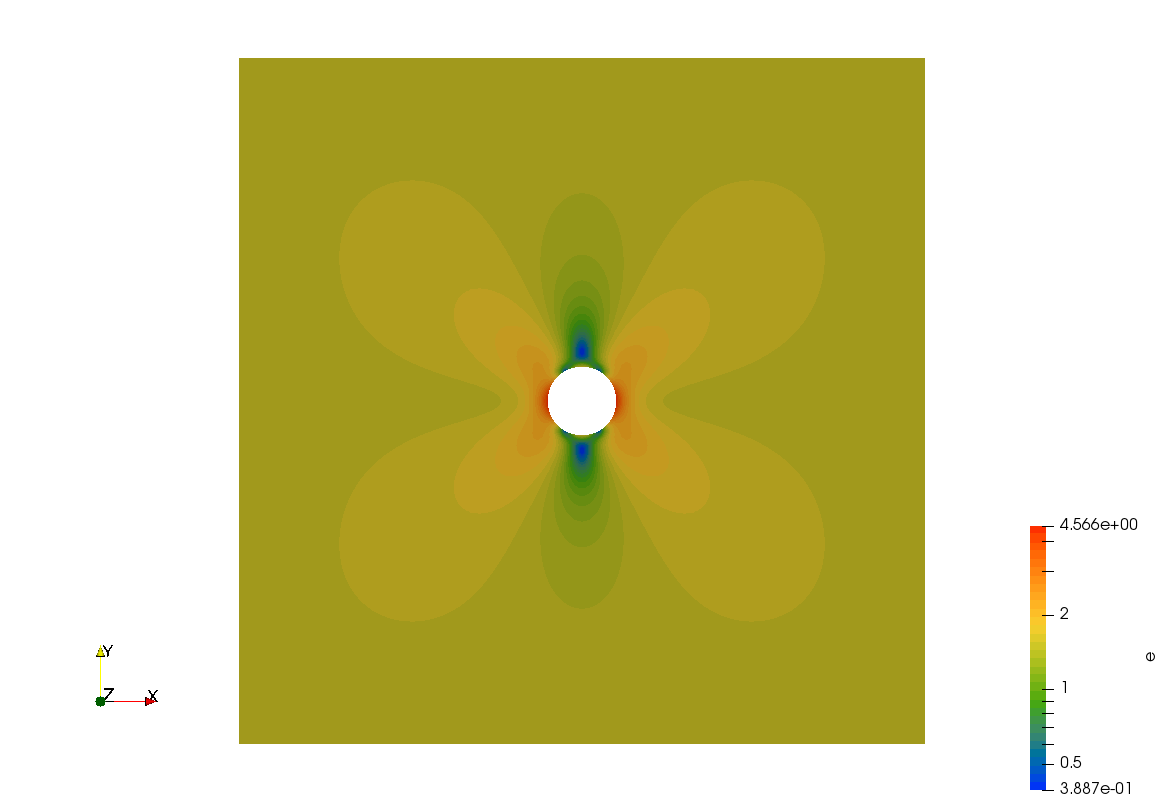
\includegraphics[width=5.6cm]{python_codes/fieldstone_124/results/exp3/e}
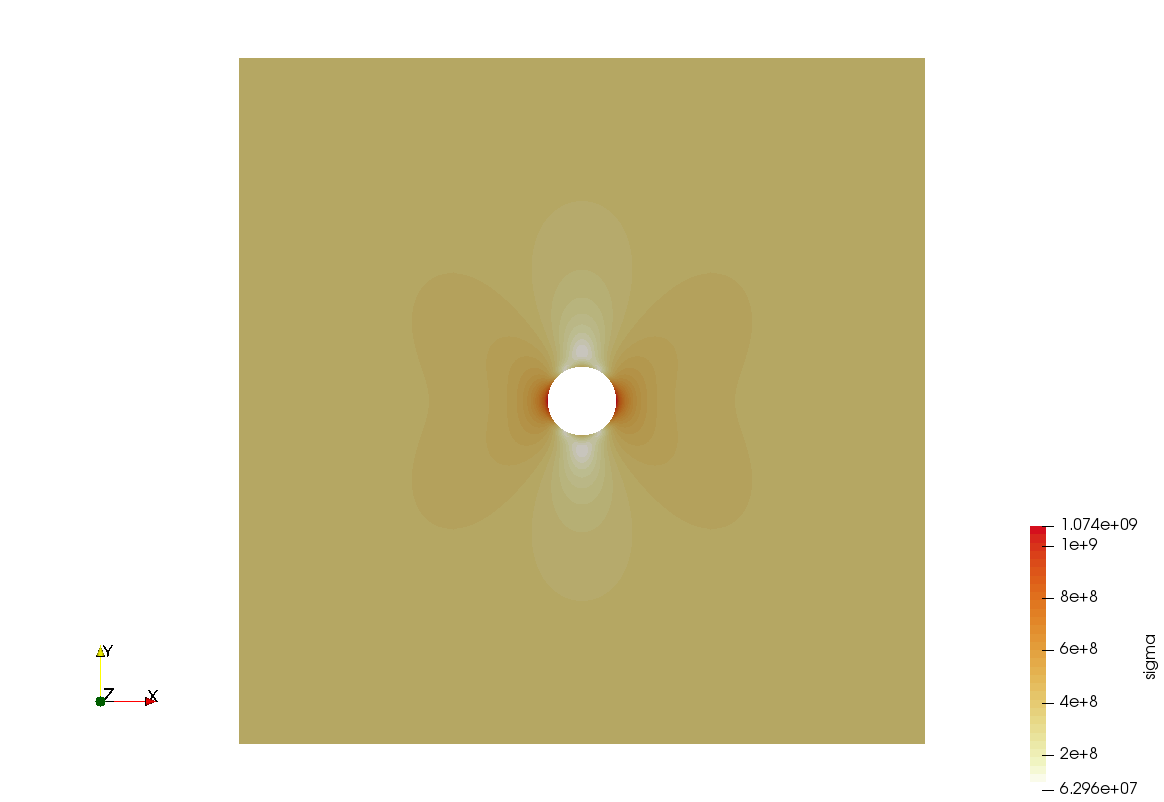
\includegraphics[width=5.6cm]{python_codes/fieldstone_124/results/exp3/sigma}\\
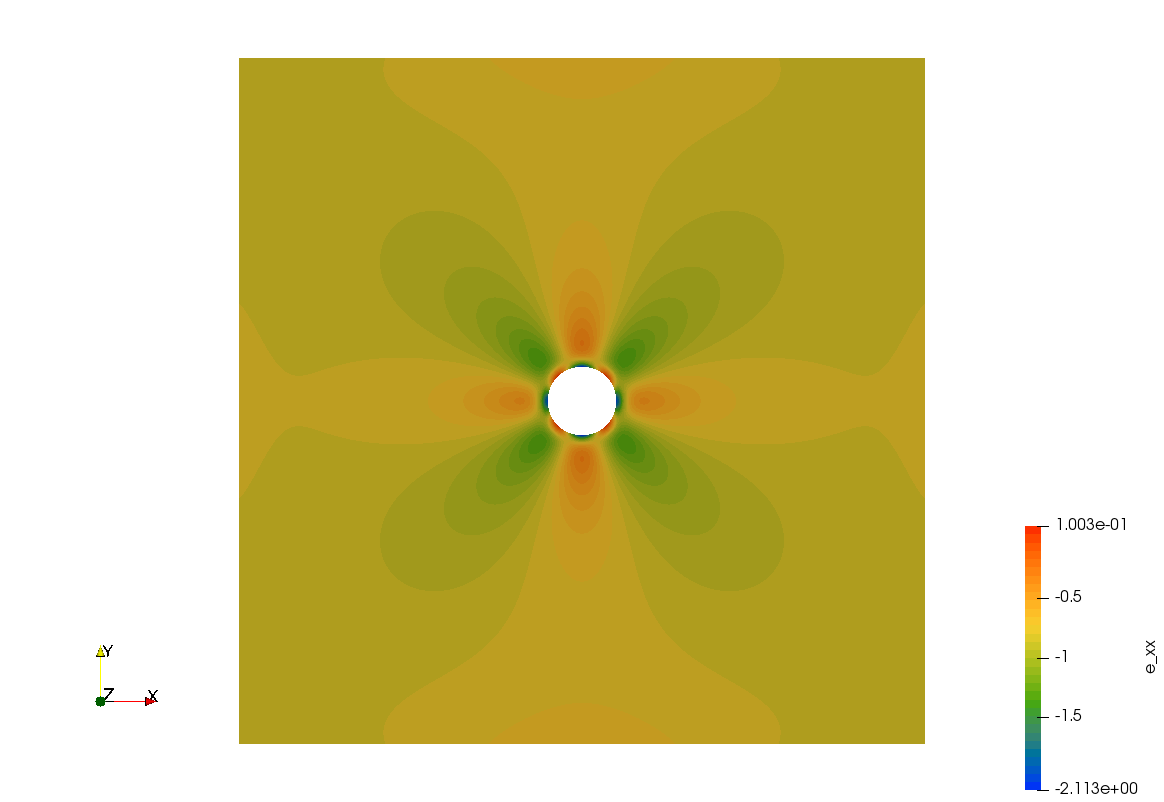
\includegraphics[width=5.6cm]{python_codes/fieldstone_124/results/exp3/exx}
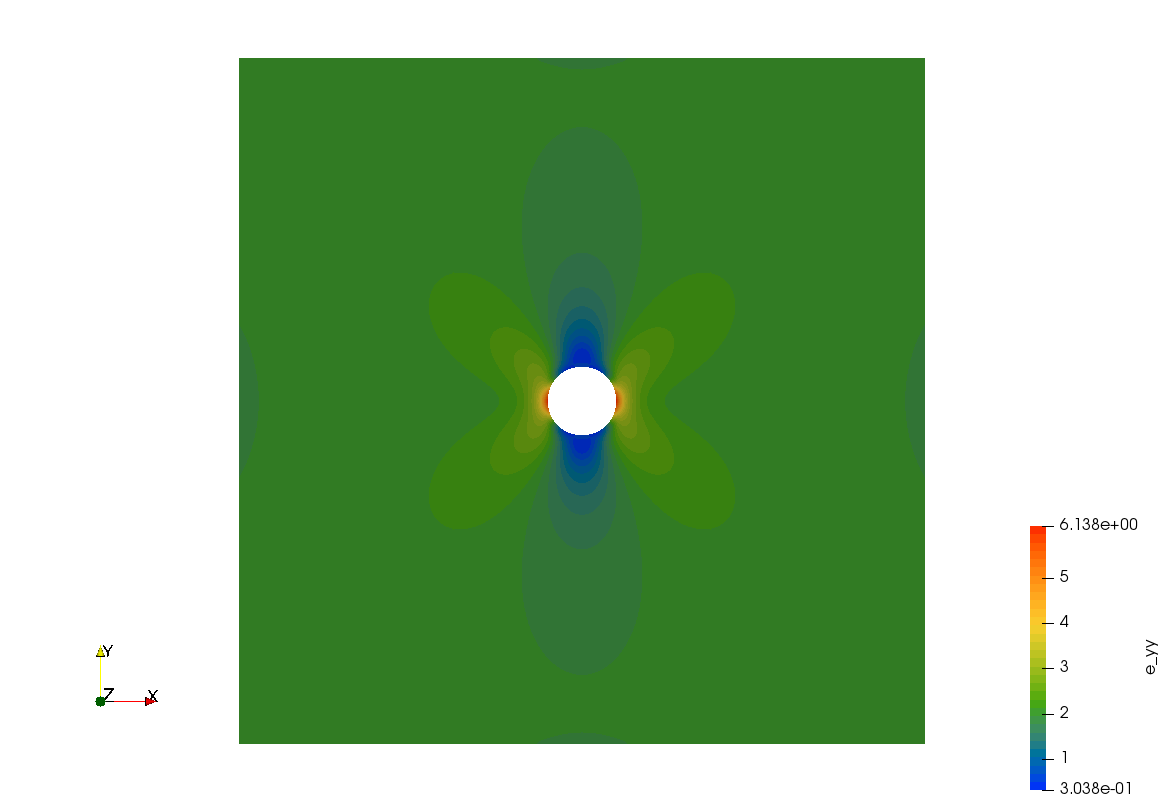
\includegraphics[width=5.6cm]{python_codes/fieldstone_124/results/exp3/eyy}
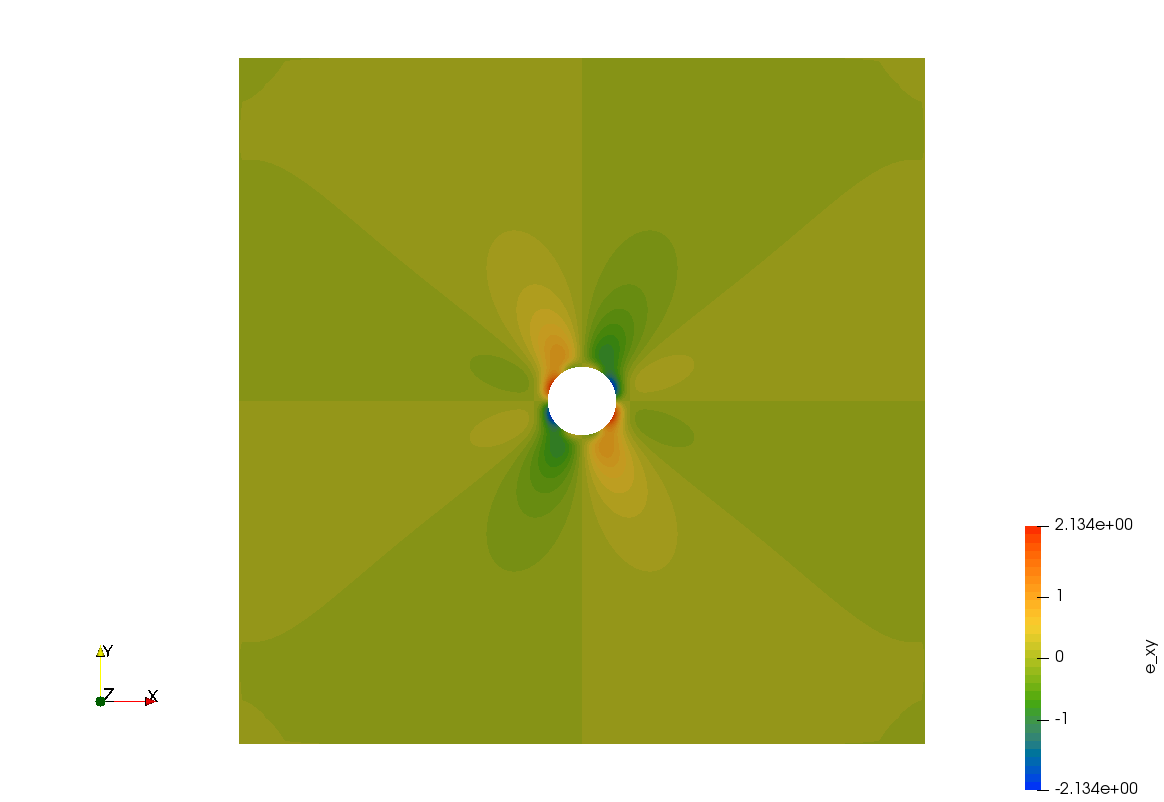
\includegraphics[width=5.6cm]{python_codes/fieldstone_124/results/exp3/exy}\\
{\captionfont Each block counts $90\times 90$ elements.}
\end{center}

The values in the above tables are now plotted against our results. 
We find a good agreement but 1) it looks like we need a {\it much higher}
high resolution to recover the published results. 
Even 8 blocks of $90\times 90$ elements each are not enough to reach a resolution-independent 
numerical solution.

\begin{center}
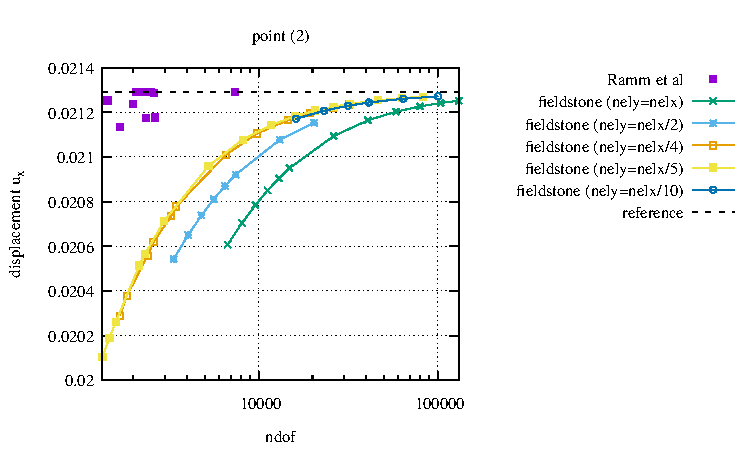
\includegraphics[width=8cm]{python_codes/fieldstone_124/results/exp3/ux2}
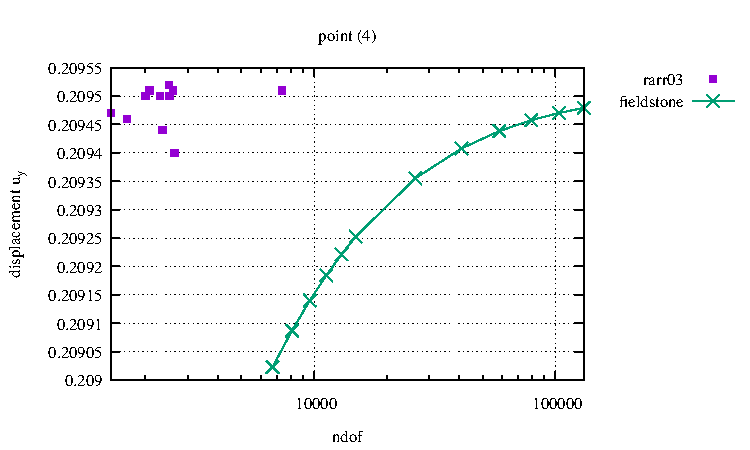
\includegraphics[width=8cm]{python_codes/fieldstone_124/results/exp3/uy4}\\
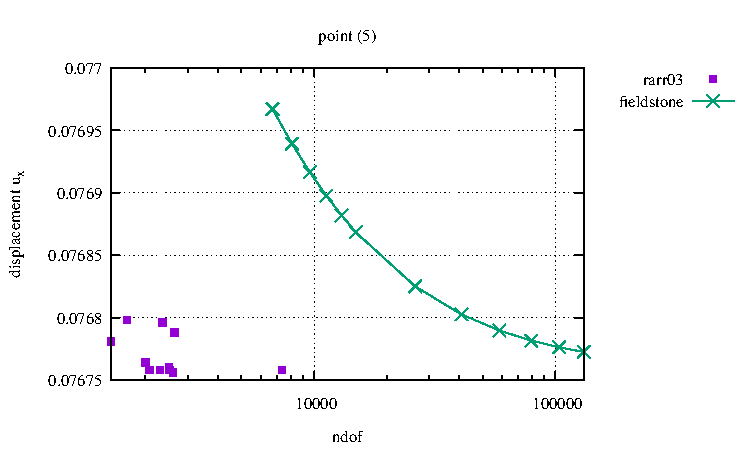
\includegraphics[width=8cm]{python_codes/fieldstone_124/results/exp3/ux5}
\includegraphics[width=8cm]{python_codes/fieldstone_124/results/exp3/sigmayy2}
\end{center}


